\chapter[A Unify Modeling of Learner's Growth Process and Flow Theory]{A Unify Modeling of Learner's Growth Process and Flow Theory}
\label{chapter:unify-modeling-learner-growth-flow-theory}

In the learning process, the affective state of students plays an essential role influencing several mechanisms of rational thinking and learning \cite{DMello2012, Picard2000, ReisRodriguezLyraJaquesBittencourtIsotani2015}.
Students with negative affective states (e.g. boredom) during the learning process are, generally, significantly more likely to obtain inadequate learning outcomes because they often are not motivated and are not engaged in the learning process \cite{CraigGraesserSullinsGholson2004, ShernoffCsikszentmihalyiSchneiderShernoff2014}.
In this sense, to motivate a student so that he/she participates in a learning scenario with complete immersion, it is necessary that his/her affective state provides an optimal experience.
This affective state is denominated flow, and it is a mental state of operation characterized by a feeling of energized focus, full involvement, and success in the task being performed \cite{Csikszentmihalyi2008}. 

To define a gamified CL scenario with game elements that favor and maintain the participants in the flow state during the CL process, it is necessary to have understanding about the influence of these game elements in the affective state of participants.
One condition for attaining and maintaining the flow state is the good balance between the perceived challenges of the tasks that will be carried out, and the participant’s own perceived abilities to accomplish these tasks.
A task that is perceived too challenging or one that is not challenging enough may lead to anxiety or boredom, and when a person perceives that he/she does not have enough ability or he/she has too ability to fulfill the task, he/she would be anxious or bored.
Thus, a model known as GMIF model: \aspas{\emph{Learner’s \textbf{G}rowth \textbf{M}odel \textbf{I}mproved by \textbf{F}low Theory}} to integrate the learner's growth process and the third condition of good balance between the perceived challenges and ability is presented in this chapter. 

This chapter is organized as follows: The first section provides details about the Learner’s Growth Model (LGM model) and the three-channel flow model (\autoref{sec:lgm-model-three-channel-flow-model}).
Then, the GMIF model is presented in \autoref{sec:integrating-learners-growth-model-flow-theory}.
To demonstrate the usefulness of the GMIF model, \autoref{sec:application-giving-rewards-by-gimf-model} illustrates how this model can be used to establish the game rewards that will be given to the participants in a gamified CL scenario to maintain them in the flow state.
Finally, \autoref{sec:model-gmif-concluding-remarks} presents the concluding remarks.

Part of the work described in this chapter was published by the author of this PhD thesis dissertation in the scientific article:

\begin{itemize}
\item
\aspas{\emph{Toward A Unified Modeling of Learner's Growth Process and Flow Theory}} published in the International Journal of Educational Technology \& Society, Vol. 19, No. 2, April 2016 \cite{ChallcoAndradeBorgesBittencourtIsotani2016}.
\end{itemize}

%%%%%%%%%%%%%%%%%%%%%%%%%%%%%%%%%%%%%%%%%%%%%%%%%%

\section{Learner’s Growth Model and Three-channel Flow Model}
\label{sec:lgm-model-three-channel-flow-model}

\subsection{Learner’s Growth Model}
\label{subsec:learners-growth-model}

Based on learning theories, the \aspas{\emph{\textbf{L}earners \textbf{G}rowth \textbf{M}odel}} (LGM model) is a graph that represents the learning process of a student as stages of skill development and knowledge acquisition as a directed graph \cite{InabaIkedaMizoguchi2003, IsotaniMizoguchi2006}.
The learner’s growth process is represented as paths on the graph that allow for the representation of the relationships between learning strategies and their educational benefits.

As shown in \autoref{fig:lgm-model}, the LGM model has twenty states that are the result of the number of stages related to skill development multiplied by the number of stages related to knowledge acquisition.
In the graph, the stages of skill development (nothing, rough cognitive, explanatory cognitive, associative, and autonomous) are represented in the lower-left triangle, while the stages of knowledge acquisition (nothing, accretion, tuning, and restructuring) are represented in the upper-right triangle.
In skill development, the cognitive stage (rough, and explanatory) involves an initial encoding of a target skill that allows the learner to present the desired behavior or, at least, some rough approximation thereof; the associative stage is the improvement of the desired skill through practice; and the autonomous stage involves gradual continued improvement in the performance of the skill \cite{Anderson1982}.
During knowledge acquisition, the accretion stage incorporates the addition and interpretation of new information in terms of pre-existent knowledge; the tuning stage involves coming to understand the knowledge through its application in a specific situation; and the restructuring stage comprises a process in which the relationship of the acquired knowledge is contemplated and the existent knowledge structure is rebuilt \cite{RumelhartNorman1976}.

The arrows in the LGM model showed in \autoref{fig:lgm-model} represent the possible transitions between stages, and the form $s(x,y)$ on the top of each vertex is the simplified form of representing a stage, where: the symbol \aspas{$x$} represents the current stage of skill development, and the symbol \aspas{$y$} represents the current stage of knowledge acquisition.
For instance, the transition $s(0,0) \to s(2,0)$ means the possible transition from the stage $s(0,0)$ where a learner does not have any knowledge or skills to the associative stage $s(2,0)$ of skill development.

 \begin{figure}[htb]
 \caption{Learner’s Growth Model (LGM model)}
 \label{fig:lgm-model}
 \centering
 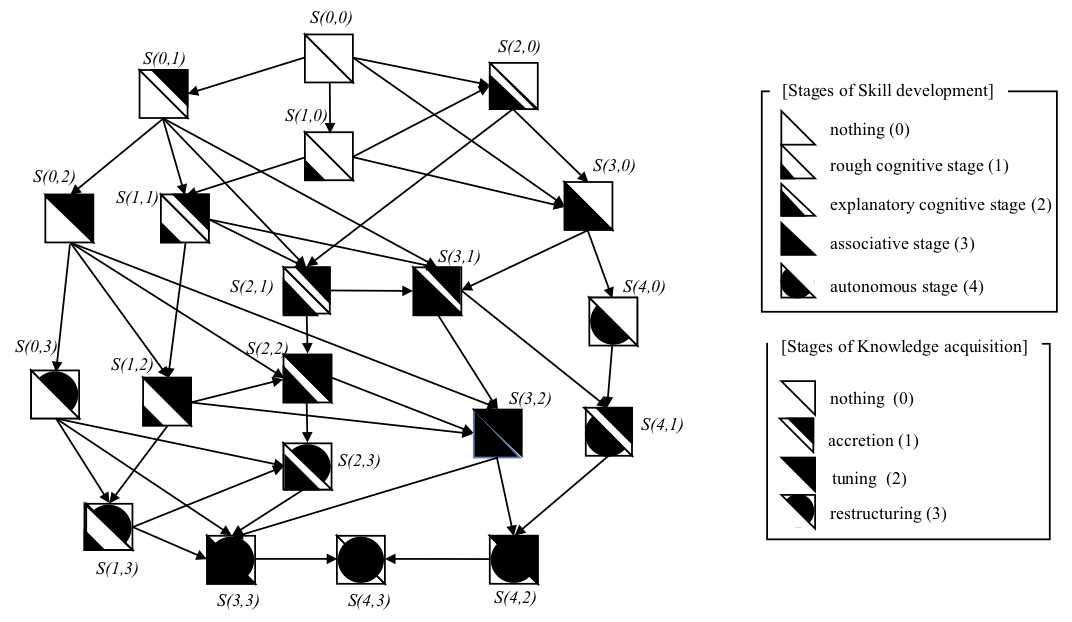
\includegraphics[width=1\textwidth]{images/chap-model-gmif/lgm-model.png}
 \fadaptada{InabaIkedaMizoguchi2003}
\end{figure}

One of the most interesting uses of this model is the representation of transitions in the skill development and knowledge acquisition stages of participants in CL scenarios based on the learning strategies employed by them and the benefits that different learning theories offer.
\autoref{fig:lgm-model-cognitiveapprenticeship} shows the representation for the transition of stages in the development of skill and acquisition of knowledge involved in a CL scenario based on the cognitive apprentice theory in which the black arrows imply the application of the learning strategies that facilitate the learner’s growth process.

 \begin{figure}[htb]
 \caption[Transitions in the LGM model for cognitive apprenticeship scenarios]{Transitions in the LGM model for cognitive apprenticeship scenarios.
 On the left side, stages in the learning by apprentice strategy for participants who play the apprentice role.
 On the right side, stages in the learning by guiding strategy for participants who play the master role}
 \label{fig:lgm-model-cognitiveapprenticeship}
 \centering
 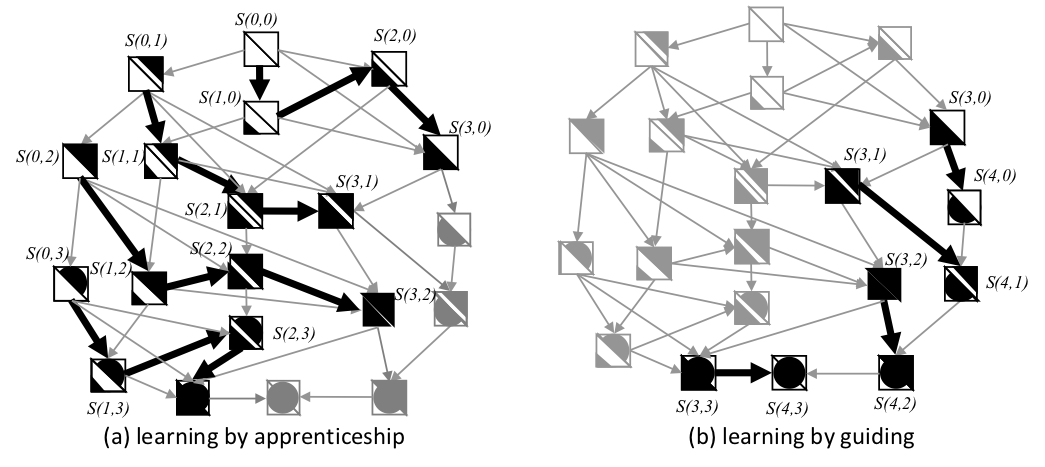
\includegraphics[width=1\textwidth]{images/chap-model-gmif/lgm-model-cognitiveapprenticeship.png}
 \fadaptada{IsotaniMizoguchiInabaIkeda2010}
\end{figure}

On the left side of \autoref{fig:lgm-model-cognitiveapprenticeship} is shown the transition of stages for the apprenticeship learning strategy, where the transition of stages in the LGM model represent the growing in cognitive skills from $s(0,y)$:\emph{nothing} into the $s(3,y)$:\emph{associative stage} through the $s(1,y)$:\emph{rough-cognitive stage} and the $s(2,y)$:\emph{explanatory-cognitive stage}.
These transitions in the skill development are transitions carried out by participants who play the apprentice role. On the right side of \autoref{fig:lgm-model-cognitiveapprenticeship} is shown the transitions of stages described by the learning strategy \aspas{\emph{learning by guiding}} in the LGM model.
According to this learning strategy, the participant who plays the master role grows in his/her cognitive skill from the $s(3,y)$:\emph{associative stage} into the $s(4,y)$:\emph{autonomous stage}.

With the use of the LGM model, any learning strategy or educational best practice can be explicitly described as a path on the graph, facilitating the understanding, visualization and utilization of the model \cite{IsotaniMizoguchiInabaIkeda2010}.

\subsection{Three-channel Flow Model}
\label{subsec:three-channel-flow-model}

\emph{Csikszentmihalyi’s flow theory} constitutes an important theory regarding to affective states of people during activities that require active work, such as discussions, exercises, and group activities \cite{Csikszentmihalyi2014,SnyderLopezPedrotti2010}.
This theory has been applied in several fields, including game design, commerce, and education.
The key concept of this theory is the \aspas{\emph{The Zone Flow}} as a situation in which a person is so engaged and focused on a particular task that he/she is completely immersed in it.
According to the flow theory, to achieve the flow state, the following conditions must be satisfied:

\begin{itemize}
\item Clear goals in which the expectations and rules are clearly discernable
\item Direct and immediate feedback in which the successes and failures of the tasks are apparent, so that behavior can be adjusted as needed
\item Good balance between the perceived ability and challenge
\end{itemize}

One of the conditions given above is that the flow state only occurs if there is a good balance between the perceived challenges of the task at hand and the learner’s own perceived ability to solve it. This means that the definition of a proper challenge (i.e. level of difficulty) is fundamental to design situations that promotes a flow state \cite{LinehanBellordKirmanMorfordRoche2014}.
Thus, Csikszentmihalyi proposes the three-channel flow model \cite{Csikszentmihalyi2008} shown in \autoref{fig:three-channel-flow-model}, in which both anxiety and boredom drive persons to frustration.
When a task is too difficult to be solved, it causes anxiety because it is perceived as too challenging or because the person’s ability level is not sufficient to solve the task.
In the same way, when a task is too easy it causes boredom because it is not challenging enough, or because the person’s ability level is too high for the task.

 \begin{figure}[htb]
 \caption{Affective states in terms of perceived ability level and challenge level, according to the three-channel flow model}
 \label{fig:three-channel-flow-model}
 \centering
 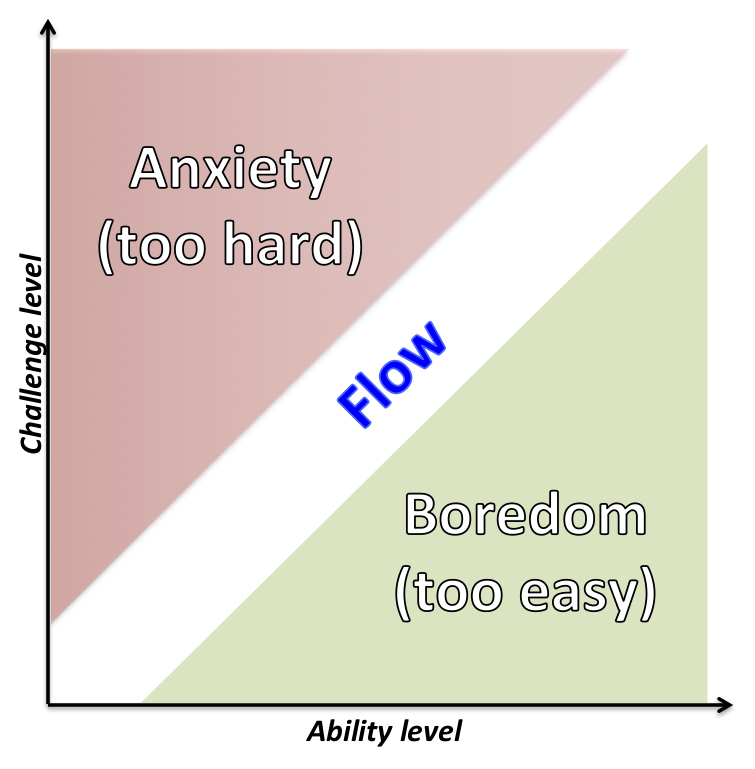
\includegraphics[width=0.5\textwidth]{images/chap-model-gmif/three-channel-flow-model.png}
 \fadaptada{Csikszentmihalyi2008}
\end{figure}

The three-channel flow model has been frequently used to build instruments and tools for the detection of the flow state \cite{KortReillyPicard2001,PearceAinleyHoward2005,Esteban-MillatMartinez-LopezHuertas-GarciaMeseguerRodriguez-Ardura2014,LeeJhengHsiao2014}.
More recently, in the context of computer education and instructional technology, studies have attempted to analyze and modeling the flow state in order: (a) to evaluate the participants’ interactions with learning objects; (b) to personalize educational activities (e.g. lessons); and (c) to develop better learning content.
In the context of game-based learning, a framework to support the integration of games as learning activities are proposed by \citeonline{delBlancoTorrenteMarchioriMartinez-OrtizMoreno-GerFernandez-Manjon2012}.
To do so, they identified key aspects about the mechanisms that facilitate the use of pedagogical approaches with games to keep students in the flow state.
Then, they proposed a workflow to integrate games into the learning process.
Therefore, this workflow can be used to create guidelines for helping instructional designers the use (and reuse) of games in the learning process.
Although this work provides some initial support for creating better learning experiences using game in the learning process, if the games themselves do not have the qualities and attributes necessary to maintain student engagement, the flow experiences will not occur.
Contemplating this problem, \citeonline{KiiliLainemadeFreitasArnab2014} proposed a framework for analyzing and designing educational games based on the flow theory.
This framework delineates several dimensions of flow experience as well as meaning factors that affect the design of game-based learning activities.


Despite the broad use of the three-channel flow model in educational contexts and its use in game-based learning, to the best of the knowledge for the author of this dissertation, there is not a computational model based on the three-channel flow model that provides support to create CL scenarios that maintain the flow state in the participants while offering theoretical justifications regarding the learner’s growth as an indicator for the perceived ability level.
Particularly, there is no computational help to define the proper levels of challenges for the game elements of a gamified CL scenario.

\section{Integrating the Learner’s Growth Model and the Three-channel Flow Model}
\label{sec:integrating-learners-growth-model-flow-theory}


The perceived challenge and ability level balance of flow theory can be determined as the current stage of the participant in the LGM model, and the challenge level to maintain the learner in the flow state.
Thus, to integrate the representation of the learner’s growth process and the condition of good balance between the perceived challenge and ability, the \emph{Learner’s \textbf{G}rowth \textbf{M}odel \textbf{I}mproved by \textbf{F}low Theory}, hereinafter referred to as GMIF model, has been proposed as a LGM model in which the arrows $s(x_{1},y_{1}) \to s(x_{2},y_{2})$ are labeling with the form $[z_{min}; z_{max}]$ to indicate the \emph{minimum challenge level} ($z_{min}$) and the \emph{maximum challenge level} ($z_{max}$) that are necessary to maintain the learner's flow.

Before to present the algorithm proposed to create a GMIF model with a n-scale of challenge level (\emph{n-scale GMIF model}), a five-scale GMIF model is presented to introduce and detail the elements involved in the building of a GMIF model.
After that, the algorithm to create a n-scale GIMF model is presented, and also, the benefits and application of GMIF model in the learning design are detailed.

\subsection{Five-scale GMIF Model}
\label{subsec:five-scale-gmif-model}

In the three-channel flow model (detailed in \autoref{subsec:three-channel-flow-model}), the levels of perceived challenge and ability are used as indicators to identify the current person's affective state in zones of anxiety, flow, and boredom. 
These two indicators are represented as axes in the three-channel flow model to depict situations where a learner is anxious, bored or in a flow state.
These situations could be represented as a rectangular region in the plane defined by the division of the perceived challenge and ability axes.
Thus, to build a GMIF model, two three-channel flow models with the division of $5 \times 5$ rectangular regions are obtained by dividing the axes into five parts.
Then, the transitions of the skill development defined by the LGM model are set to the ability axis using a uniform distribution in the first three-channel flow model to define a five-scale three-channel flow model of skill development stages and challenge levels.
In the second three-channel flow model, the transitions of the knowledge acquisition defined by the LGM model are set to the ability axis using also a uniform distribution to define a five-scale three-channel flow model of knowledge acquisition stages and challenge levels.

\begin{figure}[htb]
 \caption{Five-scale three-channel flow model of skill development}
 \label{fig:five-scale-three-channel-flow-model-skill-development}
 \centering
 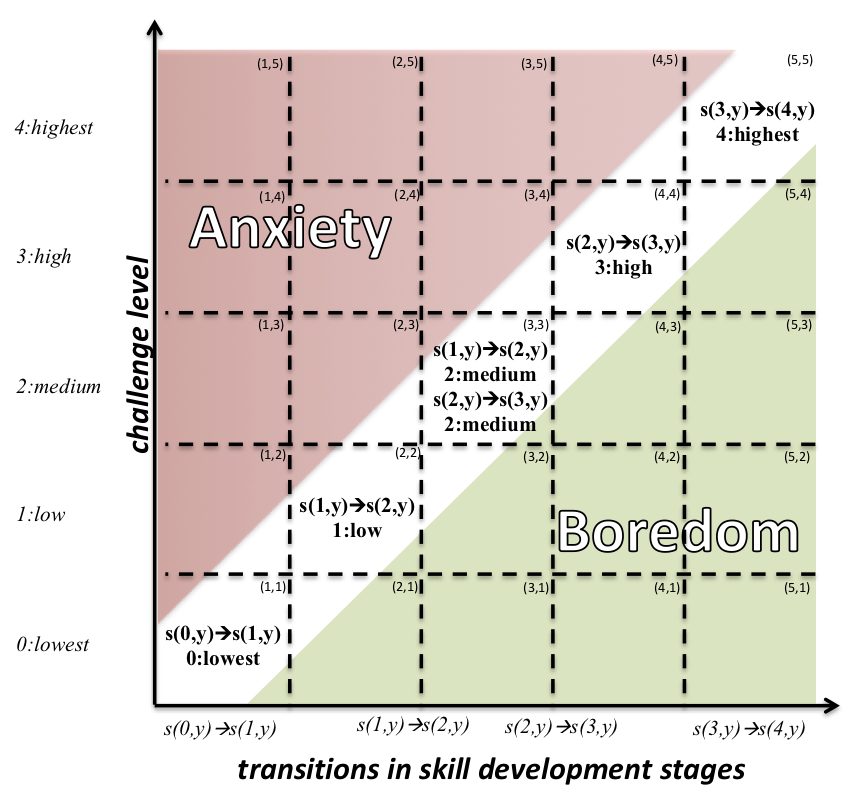
\includegraphics[width=0.65\textwidth]{images/chap-model-gmif/five-scale-three-channel-flow-model-skill-development.png}
 \fautor
\end{figure}

\autoref{fig:five-scale-three-channel-flow-model-skill-development} shows the five-scale three-channel flow model of skill development stages and challenge levels.
In this model, the five-scale challenge levels are: 0:\emph{lowest}, 1:\emph{low}, 2:\emph{medium}, 3:\emph{high}, 4:\emph{highest}.
The transitions in the skill development are: $s(0,y) \to s(1,y)$: from \emph{nothing} to \emph{rough-cognitive stage};
$s(1,y) \to s(2,y)$: from \emph{rough-cognitive stage} to \emph{explanatory-cognitive stage};
$s(2,y) \to s(3,y)$: from \emph{explanatory-cognitive stage} to \emph{associative stage};
$s(3,y) \to s(4,y)$: from \emph{associative stage} to \emph{autonomous stage}.
According to this model, the label sequences of minimum and maximum challenge levels for maintaining the learner’s flow is $s_{1}=\{[0;0], [1;2], [2;3], [4;4]\}$ in which the first element \aspas{$[0;0]$} extracted from region $(1,1)$ means that, during the transition: $s(0,y) \to s(1,y)$, the proper level of challenge to maintain the learner’s flow is 0:\emph{lowest}.
The second element \aspas{$[1;2]$} extracted from regions $(2,2)$ and $(3,3)$ means that, during the transition $s(1,y) \to s(2,y)$, the proper level of challenge to maintain the learner’s flow is in the range of 1:\emph{low} to 2:\emph{medium}. The third element \aspas{$[2;3]$} means that, during the transition $s(2,y) \to s(3,y)$ extracted from region $(3,3)$ and $(4,4)$, the proper level of challenge to maintain the learner’s flow is between 2:\emph{medium} to 3:\emph{high}.
Finally, the fourth element \aspas{$[4;4]$} extracted from region $(5,5)$ means that, during the transition $s(3,y) \to s(4,y)$, the proper level of challenge is 4:\emph{highest}.

By employing the transitions $s(x,0) \to s(x,1) \to s(x,2) \to s(x,3)$ of knowledge acquisition ($s(x,0) \to s(x,1)$: from \emph{nothing} to \emph{accretion stage}; $s(x,1) \to s(x,2)$: from the \emph{accretion stage} to \emph{tuning stage}; $s(x,2) \to s(x,3)$: from the \emph{tuning stage} to \emph{restructuring stage}), the five-scale three-channel flow model shown in \autoref{fig:five-scale-three-channel-flow-model-knowledge-acquistion} has been obtained to represent the relation of knowledge acquisition stages and challenge levels.
In this space, labels of minimum and maximum challenge levels for maintaining the learner’s flow is defined by the sequence $s_{2} = \{[0;0], [1;3], [4;4]\}$ in which the first element \aspas{$[0;0]$} extracted from the region $(1,1)$ means that means that, during the transition $s(x,0) \to s(x,1)$, the level of challenge should be 0:\emph{lowest} to maintain the learner’s flow.
The second element \aspas{$[1;3]$} extracted from regions $(1,1)$, $(2,2)$ and $(3,3)$ means that, during the transition $s(x,1) \to s(x,2)$, the proper level of challenge to maintain the learner’s flow is between the challenge levels 1:\emph{low}, 2:\emph{medium} and 3:\emph{high}.
Finally, the proper level of challenge during the transition $s(x,2) \to s(x,3)$ is 4:\emph{highest}.

 \begin{figure}[htb]
 \caption{Five-scale three-channel flow model of knowledge acquisition}
 \label{fig:five-scale-three-channel-flow-model-knowledge-acquistion}
 \centering
 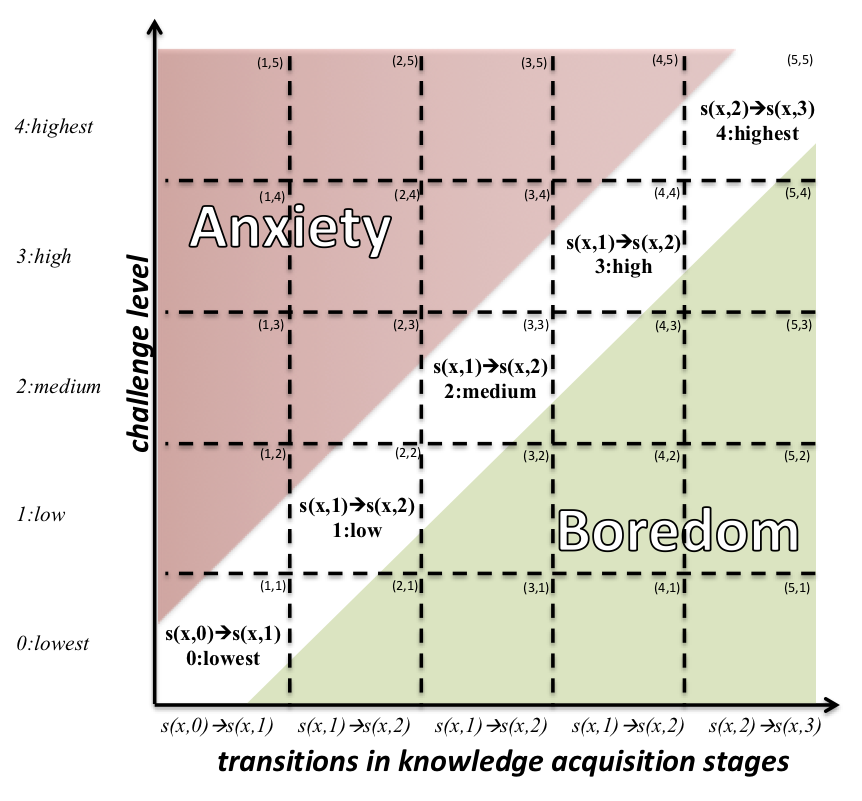
\includegraphics[width=0.65\textwidth]{images/chap-model-gmif/five-scale-three-channel-flow-model-knowledge-acquistion.png}
 \fautor
\end{figure}

To obtain the five-scale GMIF model, the relationship between the transitions of stages in the skill development and knowledge acquisition and the challenge levels should be clearly understood from the two five-scale three-channel flow models shown in \autoref{fig:five-scale-three-channel-flow-model-skill-development} and \autoref{fig:five-scale-three-channel-flow-model-knowledge-acquistion}.
With this knowledge, it is possible to design CL scenarios that (i) favor the maintenance of a flow state for students; and (ii) help them to achieve desired educational goals (i.e. acquisition of knowledge or development of skills).
To accomplish these objectives, the label sequences ($s_{1}$ and $s_{2}$) to maintain the learner's flow identified from \autoref{fig:five-scale-three-channel-flow-model-skill-development} and \autoref{fig:five-scale-three-channel-flow-model-knowledge-acquistion}, which enables us to understand when a participant is in flow state (by making the correlation between knowledge and skills with a five-scale of challenge level), to adequately label each transition (i.e. $s(x,y) \to s(x',y')$) between states in the LGM with a tuple \aspas{$[z_{min}; z_{max}]$,} where $z_{min}$ refers to the minimum challenge level necessary of to be considered interesting and not too easy, and $z_{max}$ refers to the maximum challenge level possible to be considered challenging but not too difficult.

To define the values of $z_{min}$ and $z_{max}$ in the labels \aspas{$[z_{min}; z_{max}]$} of a transition $s(x,y) \to s(x',y')$, the sequences $s_{1}$ and $s_{2}$ are used to define the proper levels of challenge for the transitions related to skill development and knowledge acquisition, respectively.
Thus, when a transition $s(x, y) \to s(x', y)$ is related to the skill development, the sequence $s_{1}$ extracted from the model shown in \autoref{fig:five-scale-three-channel-flow-model-skill-development} is used to label this transition.
For example, to develop skill from the \emph{explanatory-cognitive stage} to the \emph{associate stage}, the transition $s(2,y) \to s(3,y)$ is labeled in the LGM graph as $[2;3]$ by looking at where this transition is located in the flow area of \autoref{fig:five-scale-three-channel-flow-model-skill-development}.
In this situation, the label $[2;3]$ means that, to maintain the learner’s flow, the level of challenge for an element in the learning scenario should be selected between 2:\emph{medium} to 3:\emph{high}.
Following the same procedure, the transitions related to knowledge acquisition are used to label the transitions $s(x,y) \to s(x,y')$ defined by the sequence $s_{2}$.

\autoref{fig:five-scale-gmif-model} shows the five-scale GMIF model that results from labeling the LGM with a scale of five levels of challenge. 

 \begin{figure}[htb]
 \caption{Five-scale learner's growth model improved by the flow theory}
 \label{fig:five-scale-gmif-model}
 \centering
 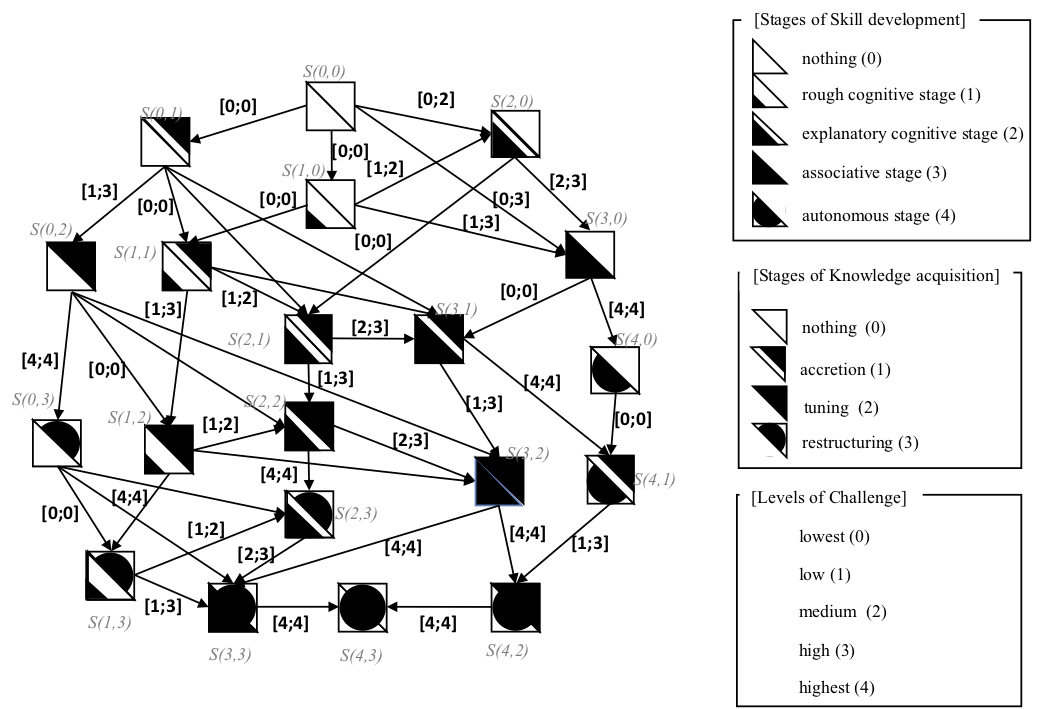
\includegraphics[width=1\textwidth]{images/chap-model-gmif/five-scale-gmif-model.png}
 \fautor
\end{figure}

\newpage
\subsection{Algorithm for Building a n-scale GMIF Model}
\label{subsec:pseudo-algorithm-n-scale-gmifs}

\autoref{algorithm:build-n-gimf-model} shows the algorithm proposed to build a GMIF model with a n-scale of challenge levels (\emph{n-scale GMIF model}), where the expected difference for the levels of challenge in the flow area is passed as the param \aspas{\emph{delta}} (as a second argument that has the default value zero).
In the algorithm, the variable GMIF contains the labels for the transitions $t = s(x,y) \to s(x’,y’)$ of the LGM model, and each label is represented as the form $[z_{min}; z_{max}]$, which indicates the minimum $z_{min}$ and maximum $z_{max}$ level of challenge that is necessary to maintain a participant is the flow state.

In the algorithm, the flow regions for the \aspas{\emph{transitions in skill development stages} vs \emph{challenge level}} and the \aspas{\emph{transitions in knowledge development stages} vs \emph{challenge level}} are obtained by the function \aspas{\emph{get\_flow\_region}} (lines 2-3), where the first parameter is the number of transitions for skill development or knowledge acquisition, and the second parameter is the n-scale of space for the challenge level, and the third parameter is the expected difference for levels of challenge.

\begin{algoritmo}
\caption{Algorithm to build a $n$-scale GMIF model}
\label{algorithm:build-n-gimf-model}
\begin{algorithmic}[1]\small
\Procedure{build\_GIMF}{n\_scale = 5, delta = 0}
  \State skill\_flow $\gets$ get\_flow\_region(4, n\_scale, delta)
  \State knowledge\_flow $\gets$ get\_flow\_region(3, n\_scale, delta)
  \ForAll{$t = (x,y) \to (x',y)$ in LGM model}
    \State GIMF[t] $\gets$ $\cup_{i=x}^{x'-1}$skill\_flow[i]
  \EndFor
  \ForAll{$t = (x,y) \to (x,y')$ in LGM model}
    \State GIMF[t] $\gets$  knowledge\_flow[y]
  \EndFor
\EndProcedure
\end{algorithmic}
\end{algoritmo}

Because the transition in the skill development stages includes flexibility that allows to increase the skill stage without following all the transitions between stages, transitions $s(x,y) \to s(x',y)$ are labeled in all levels of challenges that are defined in intermediate transitions as shown in the lines (4-6) of \autoref{algorithm:build-n-gimf-model}.
For example, it is possible to go from 0:\emph{nothing} to 3:\emph{associative stage} without moving through the intermediate stages 1:\emph{rough-cognitive stage} and 2:\emph{explanatory-cognitive stage}; thus, the transition $s(0,y) \to s(3,y)$ is labeled with the union of challenge levels defined in the transitions $s(0,y) \to s(1,y)$, $s(1,y) \to s(2,y)$ and $s(2,y) \to s(3,y)$.
For transitions related to the knowledge acquisition, the transition of stages is completed step-by-step without skipping any of the stages; thus, the transition $s(x,y) \to s(x,y')$ is labeled by setting the corresponding levels of challenge for the transitions of knowledge acquisition at shown in lines (7-9) of \autoref{algorithm:build-n-gimf-model}.

\autoref{algorithm:get-flow-region} details the algorithm for the function \aspas{\emph{get\_flow\_region}.}
This function calculates the flow region in the n-scale three-channel flow models, where the flow region is represented as an array of size $m$ (number of transitions for skill development or for knowledge acquisition) in which each $i$-th element contain the levels of challenge for the transition from the $i$-th stage to the next stage ($i+1$ stage).
For an instance of five levels of challenge and three transitions of knowledge acquisition (shown in \autoref{fig:five-scale-three-channel-flow-model-knowledge-acquistion}), the flow region as a result of the algorithm is a sequence $s = \{[0;0], [1;3], [4;4]\}$, where the first element \aspas{$[0;0]$} indicates the level of challenge as 0:\emph{lowest} for the transition $s(x,0) \to s(x,1)$.

\begin{algoritmo}
\caption{Algorithm to obtain a flow region in $m$ transitions with $n$ challenges}
\label{algorithm:get-flow-region}
\begin{algorithmic}[1]\small
\Function{get\_flow\_region}{$m$, $n\_challenges = 5$, $delta = 0$}
  \State $n \gets n\_challenges$%\LeftComment{normalize the number of challenge levels}
  \If{($n\_challenges > m$) and is.odd($n\_challenges$)}
    \State $n \gets n-1$
  \EndIf
  \State $distr \gets$ initialize\_array($m$, $\lfloor s/m \rfloor$)%\LeftComment{sets number of challenge levels for each transition}
  \State $rest \gets s - m \lfloor s/m \rfloor$
  \If{($rest > 0$)}
    \State $inv\_sigma \gets (n-rest)/2$
    \For{$i \gets 0$ to $rest-1$}
      \State $distr[inv\_sigma+i] \gets distr[inv\_sigma+i]+1$
    \EndFor
  \EndIf
  \State $flow[0].min \gets 0$%\LeftComment{make labels for flow region}
  \State $flow[0].max \gets distr[0] - 1$
  \For{$i \gets 1$ to $m-1$}
    \State $flow[i].min \gets flow[i-1].max + 1$
    \State $flow[i].max \gets flow[i-1].max + distr[i]$
    \If{($n\_challenges > m$) and is.odd($n\_challenges$)}
      \If{is.odd($m$) and ($i = \lfloor m/2 \rfloor$)}
        \State $flow[i].max \gets flow[i].max + 1$
      \EndIf
      \If{is.even($m$)}
        \If{$i = \lfloor m/2 \rfloor - 1$}
          \State $flow[i].max \gets flow[i] + 1$
        \EndIf
        \If{$i = \lfloor m/2 \rfloor$}
          \State $flow[i].min \gets flow[i] - 1$
        \EndIf
      \EndIf
  \EndIf
  \EndFor
  \ForAll{$r$ in $flow$}
    \If{($r.max = -1$)}
      \State $r.min \gets -1$
    \Else
      \State $r.min \gets r.min - delta$
      \State $r.max \gets r.max + delta$
    \EndIf
  \EndFor
  \State \Return $flow$
\EndFunction
\end{algorithmic}
\end{algoritmo}

The function \aspas{\emph{get\_flow\_region}} described as the \autoref{algorithm:get-flow-region} is summarized in a narrative form as:
Calculates the levels that should be distributed for each transition of stage (lines 2-13).
These values are calculated through a uniform distribution that tries to maintain the same number of levels in all stages.
The stages located in the same distance of the mean stage should have the same number of levels.
For example, the distribution of eight levels of challenge in five transitions is defined as the array $s = \{1,2,2,2,1\}$, where the second, third, and fourth transitions are set with two levels, it is $s(1) = s(2) = s(3) = 2$, whereas the first and fifth transitions are set with one level, it is $s(0) = s(4) = 1$.
Finally, the transition located in the third transition is set with two levels, it is $s(2) = 2$.
The steps that calculate these levels are as follows:

\begin{itemize}
\item
The normalization for the challenges levels.
This is done to avoid the non-uniform distribution that happens when the challenges levels is odd and it is greater than the number of transitions.
For example, the distribution of nine levels among four transitions only can be done by setting one transition with three levels, and setting the rest of transitions with two levels.
Therefore, the normalization for the levels of challenge is done by reducing the number of levels by one (lines 2-5).
In the previous example, the distribution of nine levels into four transitions can be defined as the array $s = \{2, 2, 3, 2\}$ before the normalization, and the distribution of these nine levels after the normalization is defined as the array $s = \{2, 2, 2, 2\}$.
\item
After the normalization, the minimum number of challenge level for each stage is defined by the function \aspas{\emph{initialize\_array}} (line 6), which initializes an array of size $m$ with the value.
The remaining levels of challenge (line 7) are distributed according to the position \aspas{$inv\_sigma$} (lines 10-12).
The value \aspas{$inv\_sigma$} is the result of dividing the number of free spaces after the distribution of the remaining challenge levels by two (line 11).
\end{itemize}

After determining the number of challenge levels that will be distributed for each transition (\emph{distr}), the next step is to set the labels for the flow region that has no contemplated difference in the levels of challenge (lines 14-32).
Thus, the process to define these labels consists in:

\begin{itemize}
\item To set the flow region for the first transition through the definition of the minimum challenge level with value zero (line 14), and the definition of the maximum challenge level with the number of challenge levels decreased by one (line 15).
\item Setting the flow region for the rest of the transitions (lines 16-32).
The minimum level of challenge is defined as the maximum challenge level of the previous transition increased by one (line 17), and the maximum challenge level is defined as the maximum challenge level of the previous transition increased by the number of challenge levels (line 18). 
For cases in which the normalization of levels has been done, the following two rules must be applied:

\begin{itemize}
\item If the number of transitions is odd, then the maximum challenge level is increased by one in the mid-transition (lines 20-22).
Thus, the flow region for nine levels of challenge in five transitions is defined as the array $s = \{[0;0], [1;2], [3;5], [6;7], [8;8]\}$.
\item If the number of transitions is even, then there are two mid-transitions:
the first mid-transition is located in the position $\lfloor m/2 \rfloor - 1$, and the second mid-transition is located in the position $\lfloor m/2 \rfloor$.
Next, the maximum challenge level is increased by one in the first mid-transition (lines 24-26). Finally, the minimum challenge level is decreased by one for the second mid-transition (lines 27-29).
Thus, the flow region for nine challenge levels in four transitions is defined as the array $s = \{[0;1], [2;4], [4;6], [7;8]\}$.
\end{itemize}
\end{itemize}

Finally, the expected difference in level of challenge, defined as the parameter delta, is used to decrease and increase the minimum and maximum levels of challenge for each transition in the flow region (lines 33-40).

\subsection{Benefits and Application of GMIF Model}

Several factors must be considered during the learning design process, such as learning goals, pedagogical preferences, intervention timing, type of feedback, students’ needs, available resources, and so on.
The work of \citeonline{KoedingerBoothKlahr2013} estimates that there is a poll of 330 (205 trillion) instructional choices that could be considered when designing a learning activity.
Unfortunately, most designers and educators do not have enough knowledge/skills to cope with this huge number of instructional choices and select those choices that are the best fit for a particular situation.
To provide help for the instructional designers in this process, the n-scale GMIF model provides a proper integration of instructional design with learning theories, models of learner’s growth, and the three-channel flow model, to reduce the complexity of the learning design task.
Specifically, the GIMF model can be used to foster flow experiences in theory-based learning scenarios.

\subsubsection*{Foster Flow Experiences in Theory-Based Learning Scenarios}

To get students into the flow state and produce optimal learning experiences, one should initially consider: 

\begin{itemize}
\item The student's initial stage and learning objectives (as final stage) in terms of knowledge acquisition and skills development \cite{Anderson1982,RumelhartNorman1976};
\item The learning path to be follow by the student based on theoretical justifications \cite{IsotaniMizoguchiInabaIkeda2010,Romiszowski1981}; and 
\item The definition of the challenge level based on the three-channel flow model.
Here it is necessary to select the necessary challenge level to keep the student in the flow state \cite{Csikszentmihalyi2014,DMello2012}. 
\end{itemize}

The GMIF model has been developed to support these steps. In the first step, the GMIF model provides a standard to delineate and represent learning objectives as well as the learner’s stage.
Thus, the problem of sharing learning designs among people and computers are reduced. Accordingly, an instructional designer can indicate the initial stage of the student and select his/her learning objectives.
Both correspond to stages in the GMIF model.
After that, the designer can check manually or automatically (using learning design authoring tools) which learning strategy based on instructional/learning theories provides an adequate learning path that supports a learner in achieving the desired goals.
In this situation, the GMIF model offers a visual representation as a sequence of arrows on the GMIF model that represents learning strategies and how they support the learner’s growth process.
Finally, to provide a flow experiences, the designer needs to define the level of challenge that is needed to maintain the student in the flow state.
In this regard, the GMIF model will indicate the level of challenge that should be considered when creating tasks to alter the state of the student while keeping him/her motivated.

%%%%%%%%%%%%%%%%%%%%%%%%%%%%%%%%%%%%%%%%%%%%%%%%%%
\section[Application of GIMF Model for the Definition of Game Rewards]{Application of GIMF Model for the Definition of Game Rewards in Gamified CL Scenarios}
\label{sec:application-giving-rewards-by-gimf-model}

With the GMIF model detailed above, we can develop different functions in authoring tools of learning scenarios.
A useful function developed by the author of this dissertation is the searching of proper learning objects that will favor and maintain the learner’s flow in the learning scenario \cite{ChallcoAndradeBorgesBittencourtIsotani2016}.
Thus, in this function, an instructional designer firstly set the initial and goal stages of a student in a learning scenario using the graphical representation of the GMIF model.
Next, each label for a difficulty level in the transition from the initial stage to the goal stage is used as a constraint to search learning objects from different repositories. 

To demonstrate the usefulness of the GIMF model in the gamification of CL scenarios, the definition of game rewards to be promised and given by game agents in gamified instructional and learning events are presented here as an application in which ontological structures to represent gamified I\_L events are used as information source.
For accomplish this task, the instructional designer first set the initial and goal stages in the graphical representation of GIMF model using the information provided by the individual goal (\emph{I-goal}) in the instructional and learning event.
Then, the learning path from the initial stage to the goal stage is identified as the learning strategy employed by the participant, and the labels of challenge levels are calculated for the arrows in the learning path according to the number of challenges/levels that could have a game component.
Finally, these labels can be used as constraints to set the game reward to be promised or given by the game agent to keep the participant in the flow state.

\begin{figure}[htb]
 \caption{Application of the GMIF model to set the game points to be given in the gamified instructional event \aspas{\emph{Gamified Checking}} of the \emph{Gamified Cognitive Apprenticeship Scenario for Master/Yee Achiever and Apprentice/Yee Achiever}}
 \label{fig:set-game-reward-gamified-checking}
 \centering
 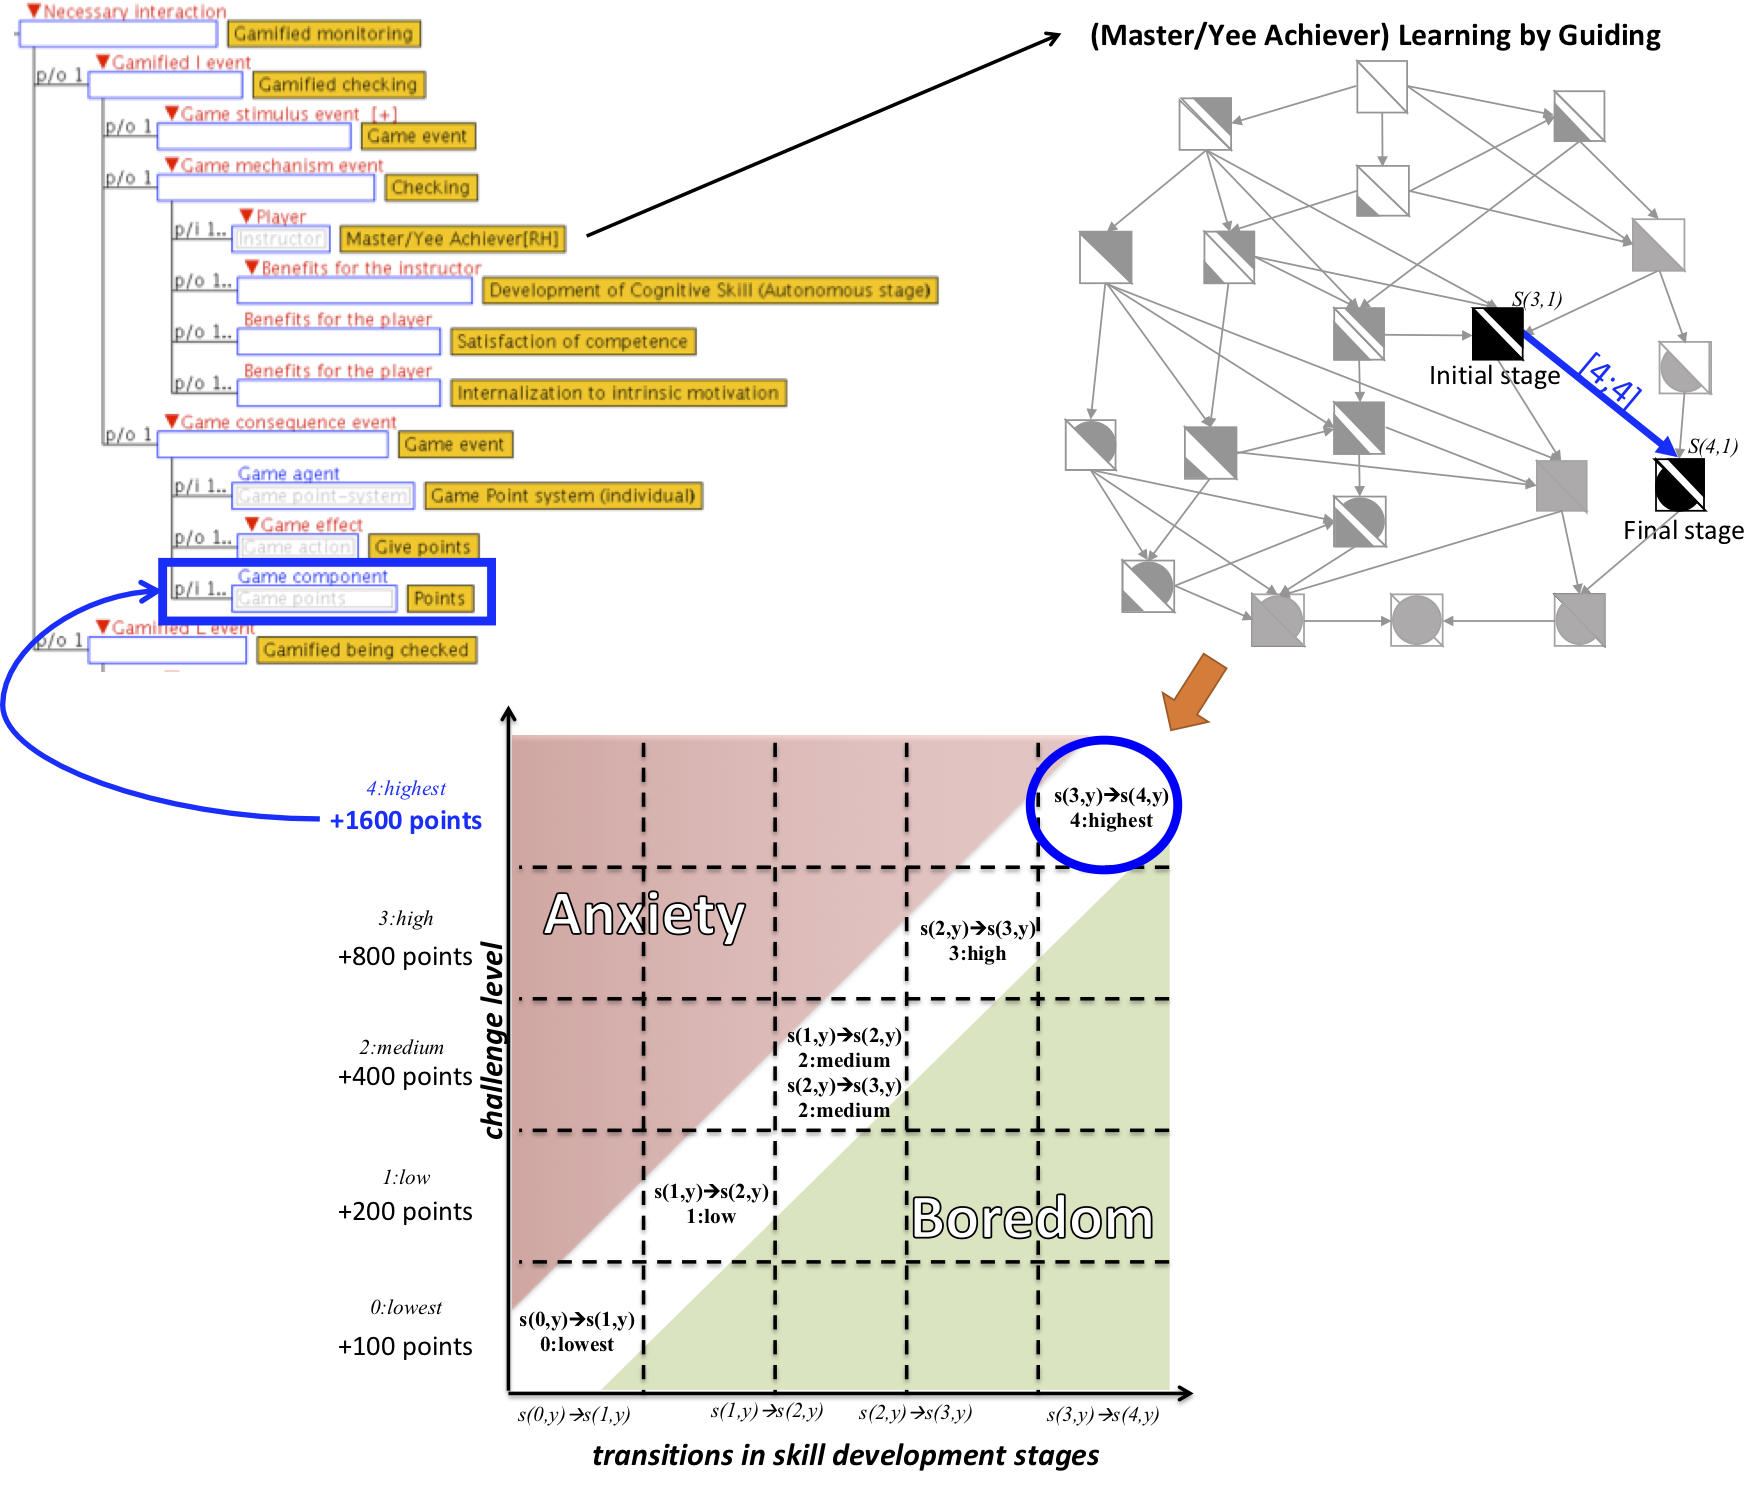
\includegraphics[width=1\textwidth]{images/chap-model-gmif/set-game-reward-gamified-checking.png}
 \fautor
\end{figure}

For the instance shown in \autoref{fig:set-game-reward-gamified-checking}, where the five-scale GMIF model has been applied to set the game points to be given by the point system as consequence of instructional event \aspas{\emph{Checking}} in a gamified CL scenario based on the cognitive apprenticeship theory with the Yee's achiever player role assigned for the master and apprentice role holder - \emph{Gamified Cognitive Apprenticeship Scenario for Master/Yee Achiever and Apprentice/Yee Achiever}.
In this situation, the instructional designer set the initial stage for the \emph{Master/Yee Achiever} role holder as $s(3,1)$ - associative stage for skill development and accretion for knowledge acquisition - and the goal stage as $s(4,1)$ - autonomous stage for skill development and accretion for knowledge acquisition.
Thus, the learning path in the GIMF model is defined by the learning strategy \aspas{\emph{Learning by Guiding},} and the proper level of challenges that will favor and maintain the \emph{Master/Yee Achiever} in the flow state is defined  by the label\aspas{$[4;4]$} that indicates a 4:\emph{highest} challenge level in the five-scale three-channel flow model of skill development stages.
Having this flow region, the proper reward to be given in the \emph{Game consequence event} by \emph{Game Point system (individual)} for the \emph{Master/Yee Achiever} role holder is \emph{+1600 points} (as \emph{Game component}).

\begin{figure}[htb]
 \caption{Application of the GMIF model to set the game points to be given in the gamified learning event \aspas{\emph{Gamified Being Checked}} of the \emph{Gamified Cognitive Apprenticeship Scenario for Master/Yee Achiever and Apprentice/Yee Achiever}}
 \label{fig:set-game-reward-gamified-being-checked}
 \centering
 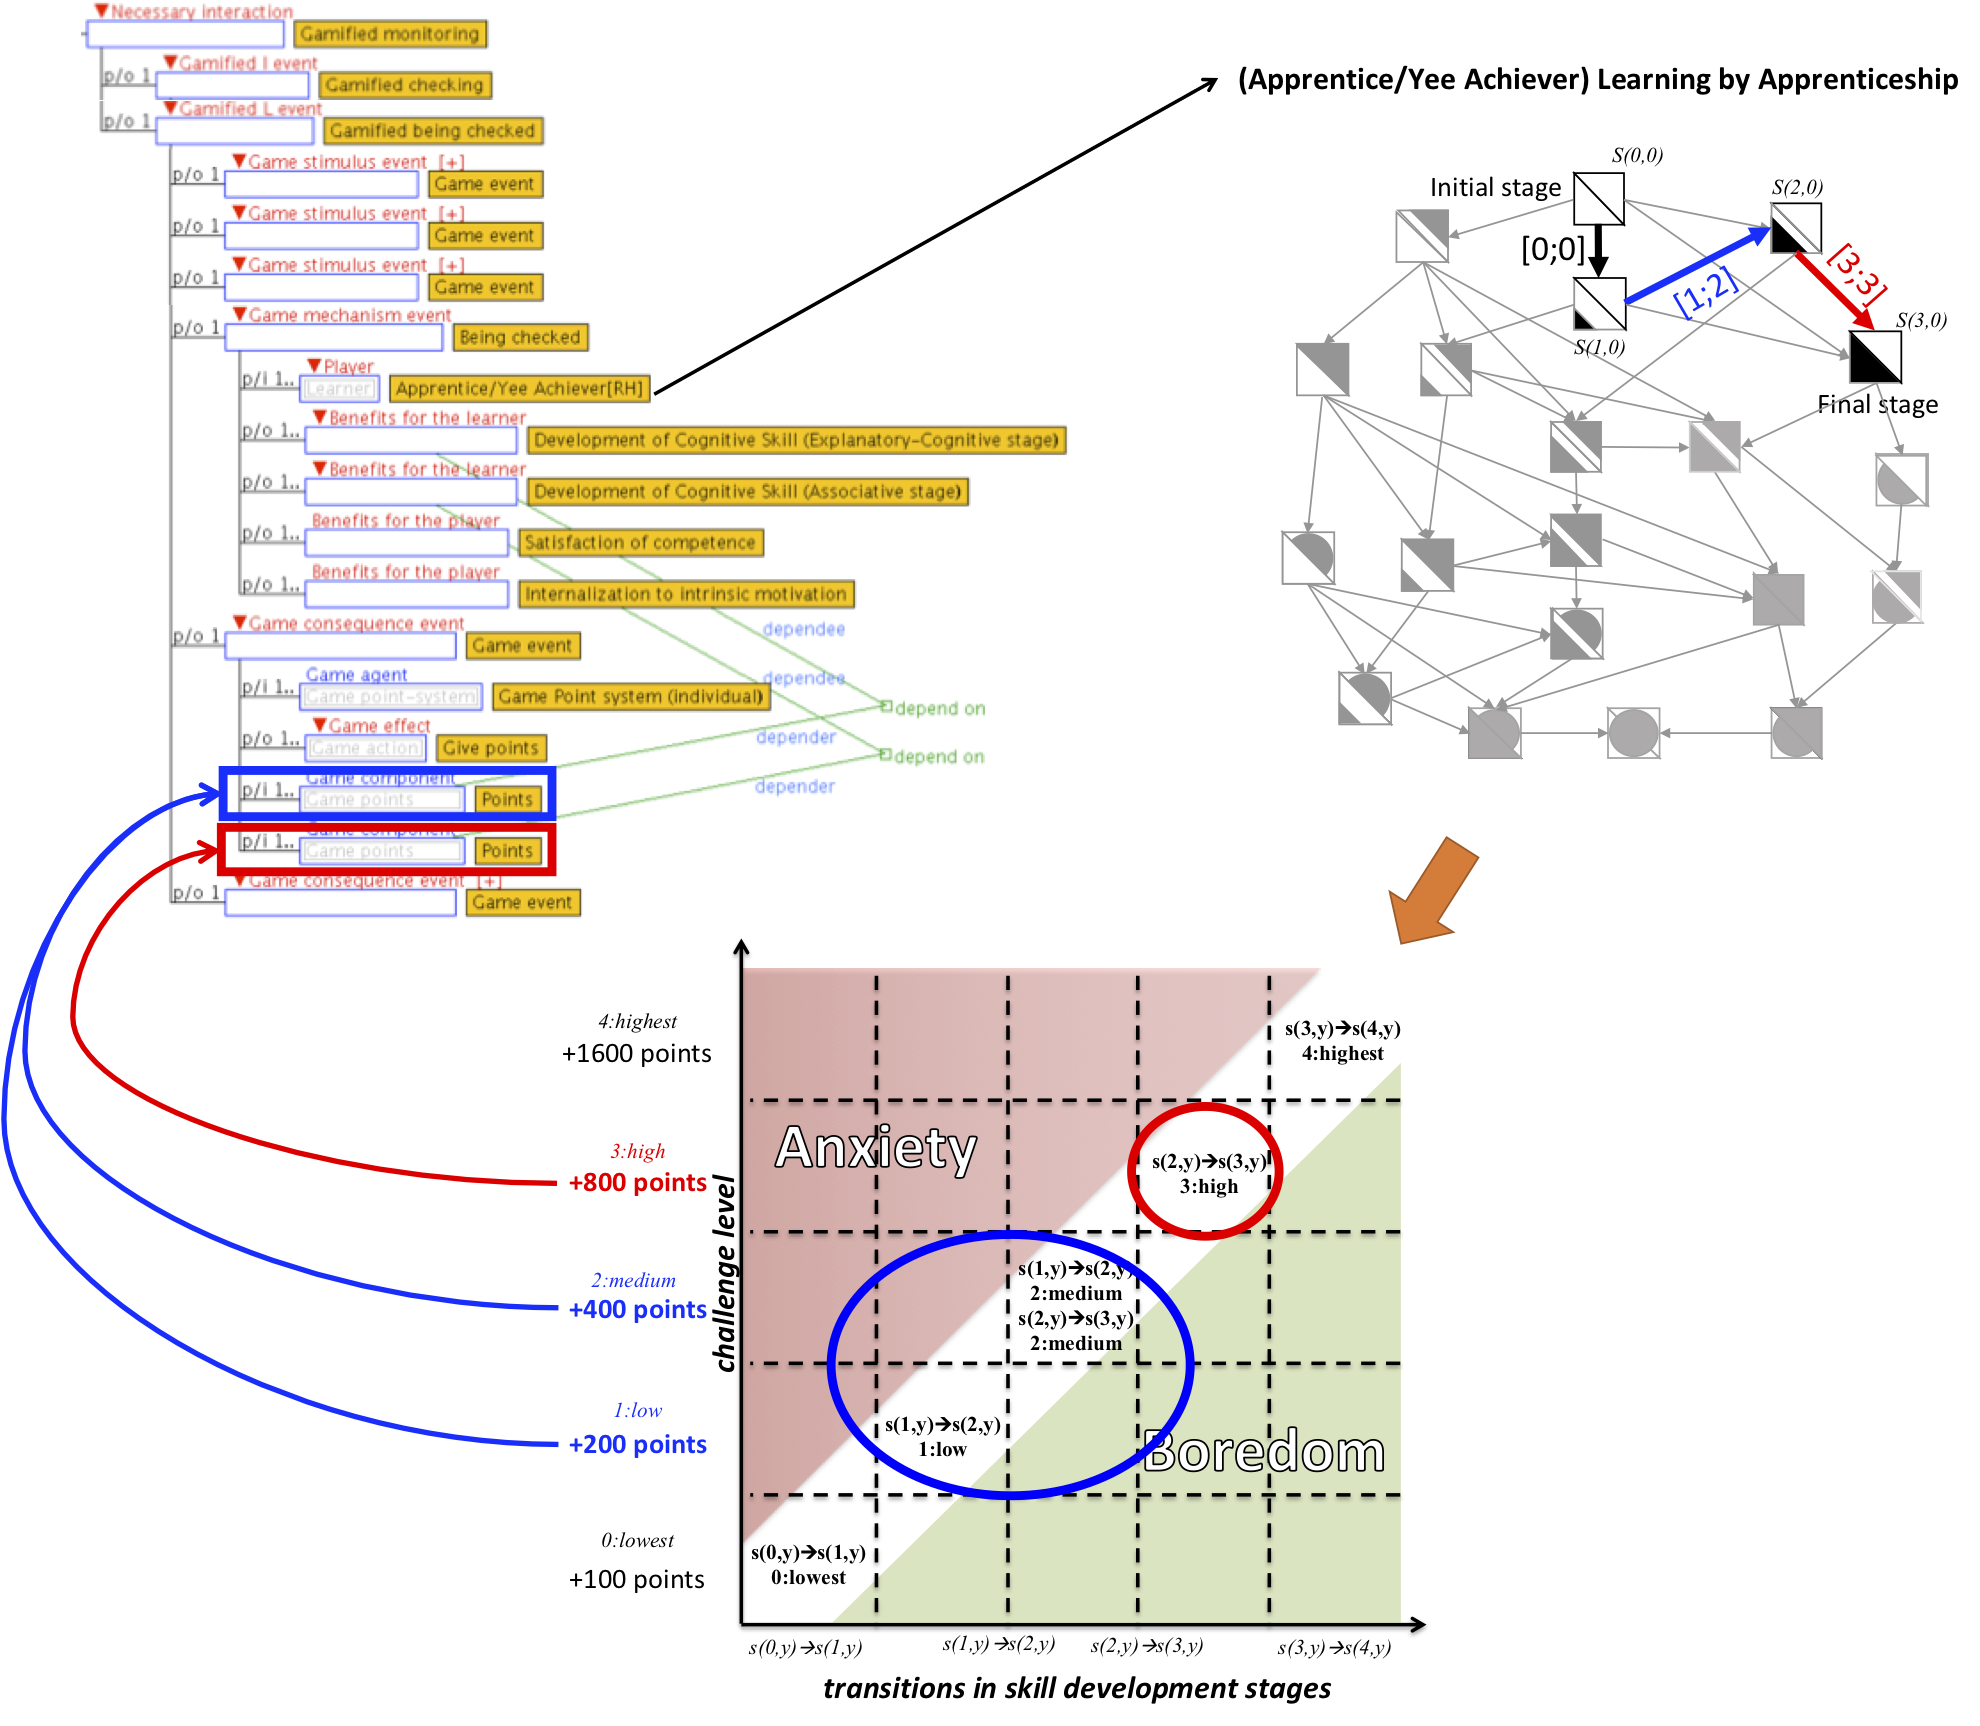
\includegraphics[width=1\textwidth]{images/chap-model-gmif/set-game-reward-gamified-being-checked.png}
 \fautor
\end{figure}

\autoref{fig:set-game-reward-gamified-being-checked} shows the application of GMIF model to set the game rewards in the gamified learning event \aspas{\emph{Gamified Being Checked}.}
In this example, the learning path identified for the \emph{Apprentice/Yee Achiever} from the initial stage $s(0,0)$ - nothing for skill development and knowledge acquisition -  to the goal stage $s(3,0)$ - associative stage for skill development and nothing for knowledge acquisition - is based on the learning strategy \aspas{\emph{Learning by Apprenticeship}.}
By the application of five-scale GMIF model, the label 
\aspas{$[1;2]$} in the transition $s(1,0) \to s(2,0)$ indicates that the proper challenges levels of 1:\emph{low} and 2:\emph{easy} are necessary to maintain the \emph{Apprentice/Yee Achiever} role holder in the flow state.
These challenge levels in the five-scale three-channel flow model of skill development stages correspond to the rewards of \emph{+200 points} or \emph{+400 points} as the game rewards that will be given by the point-system in the game consequence event when the expected benefit for the \emph{Apprentice/Yee Achiver} role holder is the \emph{Development of Cognitive Skill (Exploratory-Cognitive stage)}.
The label \aspas{$[3;3]$} in the transition $s(2,0) \to s(3,0)$ of GIMF model indicates that the challenge level to maintain the learner's flow state is 4:\emph{high}.
This challenge level corresponds to the game reward \aspas{\emph{+800 points}} as the reward to be given by the point-system to maintain him/her in the flow state during the game consequence event when the expected benefit for the \emph{Apprentice/Yee Achiever} role holder is the \emph{Development of Cognitive Skill (Associative stage)}.

%%%%%%%%%%%%%%%%%%%%%%%%%%%%%%%%%%%%%%%%%%%%%%%%%%
\section{Concluding Remarks}
\label{sec:model-gmif-concluding-remarks} 

Balancing the challenge level of elements in learning scenarios according to the current learner's ability favors the learner's flow state in those scenarios.
This balancing incorporates the flow theory in the instructional/learning design process through a theory-based model that integrates the learner's growth process and the three-channel flow model.
This new model, called GMIF model (\emph{Learner's \textbf{G}rowth \textbf{M}odel \textbf{I}mproved by \textbf{F}low Theory}), has been developed by labeling the LGM model (\emph{\textbf{L}earner's \textbf{G}rowth \textbf{M}odel}) with intervals that indicate the proper challenge levels to maintain the learner's flow state in the learning scenario.

An algorithm for labeling the LGM model with a n-scale of challenge levels, and then obtains the n-scale GMIF model, has also been proposed in this chapter.
To demonstrate the usefulness of the n-scale GIMF model, an application to set the proper level of game rewards in gamified CL scenarios has been presented.
This application has been illustrated providing support to define the points given by a point-system as game consequence events in gamified instructional and learning events.
This algorithm and the n-scale GIMF model can be used in computer-based mechanisms and procedures to support the gamification of CL scenarios that favor the learner's flow.
Furthermore, empirical studies were conducted to validate the application of GIMF model in the evaluation of the ontological engineering approach to gamify CL scenarios.
